\documentclass[10pt]{article}
\usepackage[margin=0.85in]{geometry}
\usepackage{amsmath}
\usepackage{amssymb}
\usepackage{graphicx}
\usepackage{booktabs}
\usepackage{array}
\usepackage{caption}
\usepackage{subcaption}
\usepackage[table]{xcolor}
\usepackage{hyperref}
\usepackage{enumitem}
\usepackage{placeins}
\usepackage{float}
\usepackage{microtype}
\usepackage{subcaption}
\captionsetup[subfigure]{labelformat=empty}
\usepackage{authblk}
\usepackage{titlesec}
\titlespacing*{\section}{0pt}{1.0\baselineskip}{0.4\baselineskip}
\titlespacing*{\subsection}{0pt}{0.7\baselineskip}{0.25\baselineskip}
\titlespacing*{\subsubsection}{0pt}{0.5\baselineskip}{0.2\baselineskip}
\setlength{\textfloatsep}{6pt plus 1pt minus 1pt}
\setlength{\floatsep}{6pt plus 1pt minus 1pt}
\setlength{\intextsep}{6pt plus 1pt minus 1pt}
\setlength{\abovecaptionskip}{2pt}
\setlength{\belowcaptionskip}{0pt}

\hypersetup{
  colorlinks=true,
  linkcolor=blue!55!black,
  citecolor=blue!55!black,
  urlcolor=blue!55!black
}

\captionsetup{font=small, labelfont=bf, skip=4pt}

\title{\textbf{REACH: A Reproducible Benchmark for Rare Malignant Cell
Detection in Single Cell RNA Sequencing}}

\author[1]{Moram Venkata Satya Jaswanth}
\author[1]{Amruthaluri Gavin}
\author[1]{Padarthi Aakash}
\author[1]{Muttha Tejesh Kumar}
\author[1,*]{Abhijit Dasgupta}

\affil[1]{Department of Computer Science and Engineering, SRM University, Andhra Pradesh, India}

\affil[*]{Correspondence: abhijitju06@gmail.com or abhijit.d@srmap.edu.in}
\date{}

\begin{document}
\maketitle

% -----------ABSTRACT---------
\begin{abstract}
\noindent
Rare malignant cells in single cell RNA sequencing (scRNA-seq) span
circulating tumor cells, residual disease, drug tolerant persisters, and
small malignant compartments embedded in heterogeneous tumor
microenvironments. To detect rare cells, existing methods have been evaluated inconsistently because
studies differ in datasets, label definitions, prevalence regimes, score
contracts, and failure handling. Here, we present a reproducible
benchmark framework,  Rare cell Evaluation Across Cancer Heterogeneity (REACH),  that treats rare malignant cell detection as an
imbalanced ranking task. REACH combines confidence tiered multi arm labels,
five complementary evaluation tracks (controlled real spike-ins, synthetic
splatter stress, null background controls, natural blood/CTC prevalence, and
supervised label noise diagnostics), standardized method wrappers, fallback aware
metrics, nonparametric statistics, and figure regeneration from audited
result tables. In its current form, REACH evaluates ten recent computational methods on ten curated scRNA-seq cancer datasets comprising 359,739 cells. Across 1,110 benchmark tasks, this produces 11,100 individual method performance measurements. The supervised highly variable gene logistic regression ceiling achieves near perfect separation for many tumor related labels, with a median average precision of 1.0, indicating clear gene expression differences between tumor related and non tumor cell populations. In contrast, current unsupervised ranking methods recover only part of these differences. The exploratory comparator CaSee obtains a median average precision of 0.512, whereas FiRE, the strongest ranked published detector, achieves a median average precision of 0.313. Statistical testing confirms substantial performance differences among methods on the common benchmark subset. More importantly, REACH shows that performance is highly context dependent: no single method consistently performs best across tumor types, and method behavior under ranking, null controls, and label noise cannot be adequately represented by a single summary score. These findings highlight a clear gap between supervised expression-based separability and the current performance of unsupervised rare malignant cell detection methods. All code, data, figures, and documentation required to reproduce the analysis are available in the public GitHub repository: \url{https://github.com/jaswanthmoram/reach-rarecell-benchmark}
\end{abstract}

% ------------INTRODUCTION SECTION 1----------
\section{Introduction}

Tumor samples are often highly mixed. Along with dominant malignant and non-malignant populations, they may contain small groups of cells that are biologically important but difficult to observe in bulk measurements. Single-cell RNA sequencing (scRNA-seq) allows us to look at such populations of cells separately, and to investigate tumor heterogeneity with an unprecedented level of detail \cite{papalexi2018single,tirosh2024cancer}. This is especially important when it comes to circulating tumor cells, metastatic intermediates, minimal residual disease cells, drug-tolerant persisters and small malignant compartments in the tumor microenvironment. These populations can be low-frequency, \textit{e.g.}, contribute to 1\% or less in a given dataset \cite{torre2018rare,gao2021delineating}. That not only makes them challenging to identify in biological terms, but also in statistical ones. They can be more difficult to extract if rare cells are in a more diluted cluster. If these cells are rare, mixed with neighbouring cells expressing related cell-types or have low confidence from expression and copy number evidence, they become nearly impossible to identify \cite{martens2023rarity,stegle2015computational,ren2018understanding}.

This is particularly challenging for cancer data sets where the label malignant may not be clear-cut. A cell can be classified as malignant based on copy number alteration, cancer associated expression signatures, somatic mutation evidence, neighborhood structure or expert annotations \cite{gao2021delineating,gasper2022variant,nofech2023pan}. However, in practice, the evidential sources may not be fully congruent. For some cells, there is strong evidence of expression but weak support by copy number, while others can be hard to classify if they are near non malignant populations. This sets rare malignant cell detection apart from its cousin cell-type annotation, where the expected classes are usually more clearly delineated. Moreover, the problem is extremely imbalanced as there are frequently many more background cells surrounding the malignant cells of interest \cite{johnson2019survey,altalhan2025imbalanced}.

This imbalance also raises questions about how methods should be assessed. The Area Under the Receiver Operating Characteristic Curve (AUROC) is widely used as a performance metric for machine learning classification and ranking tasks, but it becomes unwieldy and confusing if the positive class size shrinks very small. If true rare malignant cells are not ranked anywhere near the top of the list for a method, it may obtain a quite reasonable AUROC. Due to the high imbalance ratio, precision recall based measures are often more meaningful in this setting since they reflect whether rare positive cells are recovered among the highest ranked predictions \cite{davis2006relationship,saito2015precision}. However, performance should never be evaluated on just a single statistic. Changing label definition, data distribution, null behavior, method failure and statistical error makes how to interpret benchmark results a complex matter.

There have been multiple scRNA-seq benchmarks that have already been created to test batch effect correction, clustering, cell-type annotation and rare cell discovery. These benchmarks serve as useful reference standards for method comparison. Nevertheless, rare malignant-cell detection requires a more tailored assessment plan. The targeted population may be very small, the label may require multiple types of biological evidence, and the same approach may not perform uniformly across tumor types, sequencing platforms or prevalence settings \cite{tran2020benchmark,wang2022comparison,tian2019benchmarking,abdelaal2019comparison}. Thus, a benchmark for this task should not return just one best method. It should use common rules to compare methods, separate supervised reference performance from unsupervised ranking performance, log failed or unstable runs, include null control analysis, and report results in a cancer and dataset specific manner\cite{cao2021benchmark}.

We herein present \textit{Rare cell Evaluation Across Cancer Heterogeneity} (REACH), a reproducible benchmark for rare malignant cell detection in scRNA-seq data (Fig. ~\ref{fig:pipeline}). REACH formulates the detection of rare malignant cells as an imbalanced ranking problem. It is to expect that a method would give more scores to high-confidence malignant cells than to high confidence background cells. It contains the various stages of a typical pipeline, from data ingestion and preprocessing to multi evidence label construction, evaluation track generation, method execution, metric summarization and statistical analysis.

Five evaluation tracks were designed to analyze different aspects of method behavior in REACH (Fig. ~\ref{fig:tracks}). Track A evaluates real malignant cells under controlled rarity levels and serves as the primary ranking endpoint. Track B tests method performance under synthetic stress. Track C uses background-dominated controls to assess false-positive behavior when rare malignant cells are not expected. Track D evaluates natural prevalence in blood and circulating tumor cell datasets. Track E examines how the supervised ceiling changes when labels are deliberately corrupted; therefore, it is interpreted as a supervised label noise diagnostic rather than as a general robustness test for unsupervised methods. The current audited REACH snapshot includes 10 datasets, 10 methods, and 11,100 individual method performance measurements. The framework also provides instructions for adding new datasets and methods, so that it can be extended in future studies.

The results show that many high confidence malignant and background labels contain gene-expression differences that can be recovered by a supervised model. However, current unsupervised and rarity-based methods recover only part of this separation on the primary Track A endpoint \cite{abdelaal2019comparison,mahalanabis2022evaluation}. REACH also shows that method performance changes across datasets and evaluation tracks. A method that performs well in one tumor context may not remain the strongest method in another \cite{xu2024sccad,ye2025revealing}. These findings support the need for a reproducible benchmark that evaluates rare malignant-cell detection in relation to dataset context, rarity level, failure behavior, and evaluation condition.

% --------------RELATED WORK SECTION 2----------
\section{Related work}

\subsection{Rare cell discovery in scRNA-seq}

Finder of Rare Entities (FiRE) assigns a density-derived rarity score to each cell and is included in REACH as one of the ranked published comparators \cite{martens2023rarity}. The Cell Subtype Identification from Up regulated gene Sets (CellSIUS) method uses up regulated gene sets and greater specificity for rare sub populations of complex single cell populations from single cell RNA sequencing to detect rare populations \cite{wegmann2019cellsius}. The detection of rare populations using single molecule RNA fluorescence \textit{in situ} hybridization (RNA FISH) shows the dual dependence of the detection of rare expression on both the studied gene set and the number of cells from which expression is derived \cite{torre2018rare}. Further analysis of cellular expression using deep clustering and anomaly detection scorers, such as Deep Single Cell Ensemble Network Analysis (DeepScena) and single cell Clustering-based Anomaly Detection (scCAD) are starting to give the first steps of multi sample benchmarking to get an insight into the effect of pool and/or batch correction on the recovery of rare populations \cite{lei2023self,xu2024sccad}. Together, these methods motivate their inclusion in REACH, but they also show why a cancer-specific benchmark is needed: rare malignant cells may not share a single gene program and often require confirmation from multiple evidence arms \cite{tirosh2024cancer,ren2018understanding}.

\subsection{Single cell benchmarking}

Various mixture control tests have been used to benchmark a number of different scRNA-seq pipelines \cite{tian2019benchmarking}. Other studies have provided benchmarking of cell type classification, batch corrections, clustering for tumor types in cancer, automated annotation of tumor cells  and copy number inference \cite{abdelaal2019comparison,tran2020benchmark,mahalanabis2022evaluation,chen2025benchmarking,christensen2023evaluation}. These studies established useful practices for benchmarking fixed datasets with clearly defined metrics. However, the low frequency of detection for the presence of malignant cells required prevalence adjusted methods, null controls, fallbacks and ranked metrics, based on the previous template \cite{davis2006relationship,saito2015precision,johnson2019survey}.

\subsection{Malignant cell annotation and CNV evidence}

Labeling of malignant cells is typically done using the combined results of expression and copy number variation (CNV) inference \cite{gao2021delineating}. Copy number Karyotyping of Tumors (CopyKAT) can delineate copy number and clonal substructures \cite{gao2021delineating}. Moreover, single cell Annotation of Tumor and Immune Cells (scATOMIC) assigns cell types to the cells in the tumor microenvironment for all types of cancer \cite{nofech2023pan}. Here, variant calling has been tested as another way of providing evidence of the presence of a cancer cell \cite{gasper2022variant}. REACH uses CNV and cancer signature evidence to support label construction rather than to create a separate leaderboard score. In other words, these signals help define high confidence malignant and background cells, but they are not themselves ranked as competing detection methods. Candidate methods that failed to provide valid cell level scores or did not satisfy the required score contract are documented in the method inclusion audit and excluded from the main ranking analyses (Fig.~\ref{fig:fig3}(a)).

% -------------METHODOLOGY SECTION 3----------
\section{Methodology}

\subsection{Task definition and metrics}

For benchmark unit $u$, let $X_u\in\mathbb{R}^{n_u\times p}$ be the
log normalized expression matrix, where
$n_u$ denotes the number of cells and $p$ the number of genes in unit $u$.
Let $y_{ui}\in\{0,1\}$ denote the ground truth label of cell $i$ in unit
$u$, where $y_{ui}=1$ indicates a high confidence malignant (rare cell)
state and $y_{ui}=0$ indicates background or non malignant status.
A method $m$ returns a continuous cell level score
\begin{equation}
  f_m(X_u) = s_u^{(m)} \in \mathbb{R}^{n_u},
\end{equation}
where $s_u^{(m)}$ is the vector of predicted scores for all cells in unit
$u$, and larger scores indicate stronger predicted malignant or rare cell
status. REACH evaluates ranking performance rather than thresholded
diagnosis.
For a ranked list, the standard interpolated Average Precision
(AP)~\cite{davis2006relationship,cormack2006statistical} is
\begin{equation}
  \mathrm{AP}(m,u) \;=\; \sum_{k=1}^{n_u}\!\bigl(R_k - R_{k-1}\bigr)\,P_k,
\end{equation}
where $P_k$ and $R_k$ denote precision and recall after the first $k$
ranked cells, respectively, with $R_0 = 0$.
The primary method summary is the median Track A AP
computed across all valid benchmark units,
\begin{equation}
  S_m \;=\;
  \mathop{\mathrm{median}}_{u\in\mathcal{U}_{A,m}^{\mathrm{valid}}}
  \mathrm{AP}(m,u),
\end{equation}
where $\mathcal{U}_{A,m}^{\mathrm{valid}}$ denotes the set of Track A
benchmark units that remain after fallback-based filtering for method $m$.
Because raw AP depends on class prevalence, REACH additionally reports
prevalence adjusted quantities. Let
\begin{equation}
  \pi_u = \frac{1}{n_u}\sum_i y_{ui}
\end{equation}
denotes the positive class prevalence in the benchmark unit $u$. AP above
chance is defined as $\mathrm{AP}(m,u)-\pi_u$, and the normalized AP is
\begin{equation}
  \mathrm{nAP}(m,u)
  \;=\;
  \frac{\mathrm{AP}(m,u)-\pi_u}{1-\pi_u}.
\end{equation}
AUROC is reported as a secondary discrimination
metric~\cite{davis2006relationship,saito2015precision}. Calibration
metrics, including the Brier score and Expected Calibration Error (ECE),
are reported only for probability like outputs and are explicitly marked
as \emph{not applicable} for rank-based or anomaly-based scores. F1,
precision, recall, balanced accuracy, and Matthews correlation coefficient
(MCC) are reported at top $k$, where $k$ equals the number of positive
cells in the corresponding benchmark
unit~\cite{johnson2019survey,altalhan2025imbalanced}.


\begin{figure}[H]
\centering
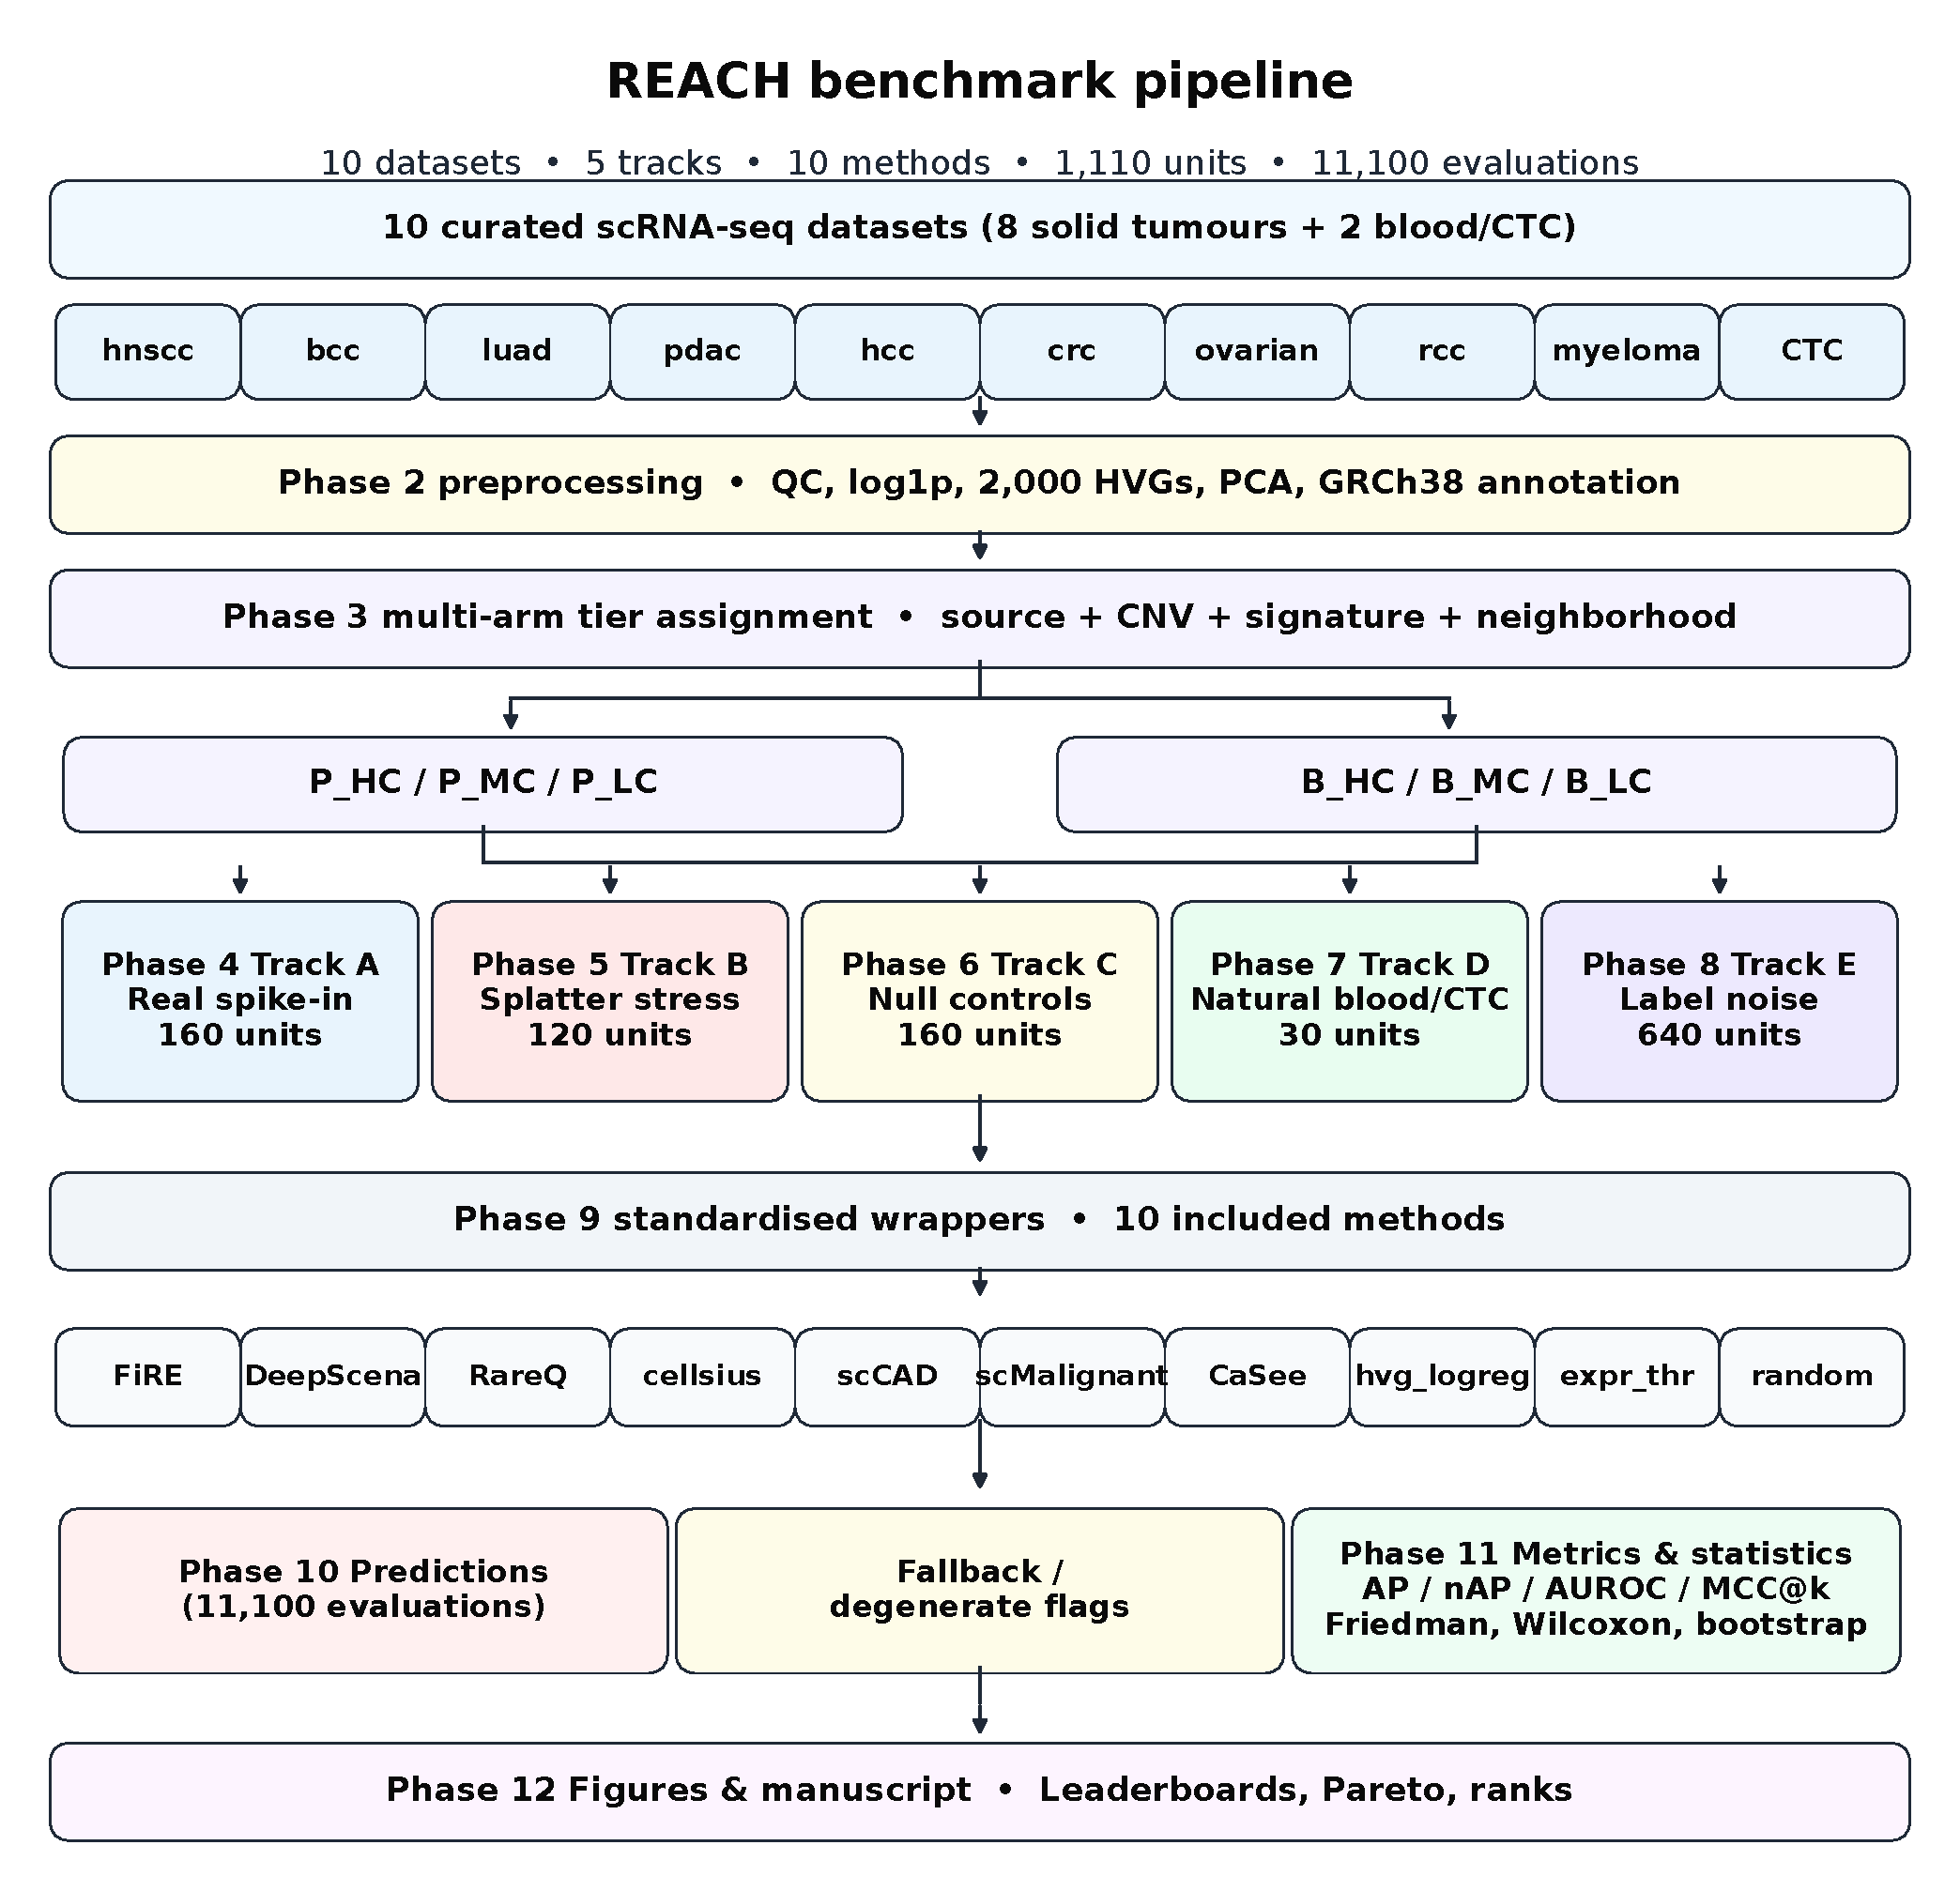
\includegraphics[
width=0.97\linewidth,
height=0.78\textheight,
keepaspectratio
]{figures_final/Fig1_REACH_Pipeline_Overview.pdf}
\caption{\textbf{REACH benchmark pipeline.} Ten curated scRNA-seq
datasets are ingested, preprocessed, assigned confidence tiered
malignant/background labels, transformed into five evaluation tracks
(A to E), evaluated through standardized wrappers for ten methods, and
summarized by metrics, statistical tests, and publication figures. Each method is evaluated on 1,110 benchmark units, yielding 11,100 method-unit evaluations across ten methods. The
schematic mirrors the Phase~0 to 12 file contracts documented in
\texttt{docs/architecure.md}.}
\label{fig:pipeline}
\end{figure}

\subsection{REACH pipeline}

REACH is implemented as a 12-phase reproducible pipeline, beginning with environment setup and ending with audited result tables and publication-ready figures (Fig.~\ref{fig:pipeline}). Phase 0 defines the software environment, directory structure, configuration files, and execution requirements. Phase 1 collects dataset metadata and source files. Phase 2 performs standardized preprocessing, including quality control, normalization, highly variable gene selection, dimensionality reduction, graph construction, and harmonization of cell and gene annotations. Phase 3 assigns confidence tiers to cells by combining source annotations, CNV evidence, cancer-signature scores, and neighborhood support.

Phases 4--8 generate the benchmark units used for evaluation. Phase 4 creates Track A units for controlled real-cell rarity. Phase 5 creates Track B units for synthetic stress testing. Phase 6 creates Track C background-dominated null-control units. Phase 7 creates Track D units using natural blood and circulating tumor cell prevalence. Phase 8 creates Track E units for supervised label-noise analysis by keeping the expression matrix fixed while perturbing labels. These phases convert the processed datasets and confidence labels into fixed benchmark units with expression matrices, cell-level labels where applicable, prevalence information, and metadata.

The later phases execute and summarize the benchmark. Phase 9 runs each method through a standardized wrapper and records cell-level scores, runtime information, fidelity status, fallback flags, and degenerate-output flags. Phase 10 collects the prediction outputs across all method--unit combinations. Phase 11 computes ranking metrics, null-control summaries, runtime summaries, and statistical tests. Finally, Phase 12 regenerates the figures and manuscript-level result tables directly from the audited outputs. This phase-based design makes the benchmark traceable, because each result can be linked back to its input data, configuration files, and upstream processing contract \cite{cao2021benchmark}.


\subsection{Datasets and preprocessing}

Here, we have processed 10 datasets (Table 1), such as 8 solid tumor and 2 blood/Circulating Tumor Cells (CTC). Track A (ranking of solid tumor samples) has been done using the 8 solid tumor datasets, while Track D (natural prevalence) has been created using the 2 blood/CTC datasets. Each of the data sets has been processed through a standard AnnData pipeline \cite{jovic2022single} which includes: loading each data set, standardizing the gene symbol to the normalization standard, obtaining the mitochondrial annotations, performing hard Quality Control (QC) (minimum genes = 200; minimum Unique Molecular Identifiers (UMI) = 500; minimum cells = 3), performing the Scrublet doublet detection algorithm \cite{jovic2022single}, where possible, adaptively flagging mitochondrial results, performing total count normalization (to 10,000) with subsequent $log 1p$ transformation, providing both raw and normalized layers\cite{tran2020benchmark}, identifying the 2,000 highly variable genes (hvg) (using Seurat V3 or Cell Ranger as fallback) \cite{tran2020benchmark,abdelaal2019comparison}, calculating 50 components of Principal Component Analysis (PCA), constructing a neighborhood graph \& performing Leiden clustering (with res = 0.5 \& seed 42) \cite{mahalanabis2022evaluation}, analyzing the chromosome annotations based on the Genome Reference Consortium Human Build 38 (GRCh38) reference, standardizing the observation columns across all data sets, and finally creating gzipped .h5ad files and Secure Hash Algorithm 256-bit (SHA 256) metadata \cite{cao2021benchmark}.

\subsection{Multi arm label construction}

All cells acquire a confidence level as an outcome of the source annotation combined with a Python/Scanpy-based tool (infercnvpy CNV inference), Area Under the Curve Cell scoring (AUCell) signatures ($\geq 0.15$) and the neighborhood support ($\geq50\%$ of the $k=15$ -PCA nearest neighbours share provisional class) of the individual cells\cite{chen2025benchmarking,gao2021delineating,hetzel2021graph,fa2026cell}. All the data sets used infercnvpy as the main tool of CNV inference. CopyKAT was not used as the primary CNV-calling method because it failed the cell-level score contract and, by design, does not allow a consistent primary wrapper to be applied across different datasets \cite{chen2025benchmarking}. As a member of the Positive High Confidence (PHC), a cell should satisfy all four positive evidence criteria, such as source positive, aneuploid, high signature, and neighborhood support. The same four criteria should be in the opposite direction for the Background High Confidence (BHC) group. Here, primary AP has been computed using a subset of PHC and BHC cells. Such a design balances two goals, including enough cells for evaluation while maintaining stable and reliable high-confidence labels \cite{stegle2015computational,abdelaal2019comparison}.

\subsection{Evaluation tracks}

We use five tracks in the REACH pipeline (Fig.~\ref{fig:tracks} and Table 2). The first track (Track A) involves the use of real PHC cells sampled from a mock version of the true background by four different levels of prevalence (T1 $5$--$10\%$, T2 $1$--$5\%$, T3 $0.1$--$1\%$, T4 $0.01$--$0.1\%$)  with an aim to find around 2000 cells per unit and less than 20\% duplicates \cite{johnson2019survey,altalhan2025imbalanced}. The second one (Track B) uses Splatter simulations which are fitted to the real data and audited for library size, dropout and differential expression overlap or PCA plots \cite{cao2021benchmark}. The third track (Track C) uses only background samples (null behavior) \cite{torre2018rare}. The fourth track (Track D) uses the natural prevalence of the MM Ledergor and breast CTC Szczerba \cite{peng2019single,qian2020pan}. Track E has Track A expression matrices fixed and measures 4 corrupted label conditions (10\% symmetric flip, 20\% symmetric flip, 30\% positive→background, 30\% background→positive). Thus, the labeling procedure itself does not consume benchmark labels and is therefore not supervised in the strict sense. However, Track E should be interpreted as a supervised hvg–logistic regression (logreg) ceiling only when the evaluation is performed using the corresponding hvg-based logreg method \cite{mahalanabis2022evaluation}.

\begin{table}[H]
\centering
\caption{\textbf{Datasets}. Final cell counts follow
the Phase~1 to 12 report and are internally consistent with the tier count
table. GEO accessions are listed in the section \emph{Data and Code Availability}.}
\label{tab:datasets}
\small
\begin{tabular}{llllr}
\toprule
Dataset ID & Cancer type & Platform & Tracks & Final cells \\
\midrule
\texttt{hnscc\_puram}        & Head and neck SCC                & Smart-seq2   & A/B/C/E & 5{,}902 \\
\texttt{ov\_izar\_tirosh}    & Ovarian cancer ascites           & 10x Chromium & A/B/C/E & 9{,}482 \\
\texttt{hcc\_wei}            & Hepatocellular carcinoma         & 10x Chromium & A/B/C/E & 19{,}382 \\
\texttt{luad\_laughney}      & Lung adenocarcinoma              & 10x Chromium & A/B/C/E & 33{,}782 \\
\texttt{rcc\_multi}          & Renal cell carcinoma             & 10x Chromium & A/B/C/E & 33{,}574 \\
\texttt{pdac\_peng}          & Pancreatic ductal adenocarcinoma & 10x Chromium & A/B/C/E & 123{,}488 \\
\texttt{crc\_lee}            & Colorectal cancer                & 10x Chromium & A/B/C/E & 55{,}551 \\
\texttt{bcc\_yost}           & Basal cell carcinoma             & 10x Chromium & A/B/C/E & $\sim$47{,}000 \\
\texttt{mm\_ledergor}        & Multiple myeloma                  & 10x Chromium & D       & 31{,}181 \\
\texttt{breast\_ctc\_szczerba} & Breast cancer CTCs             & Smart-seq2    & D       & 357 \\
\bottomrule
\end{tabular}
\end{table}

\begin{figure}[H]
\centering
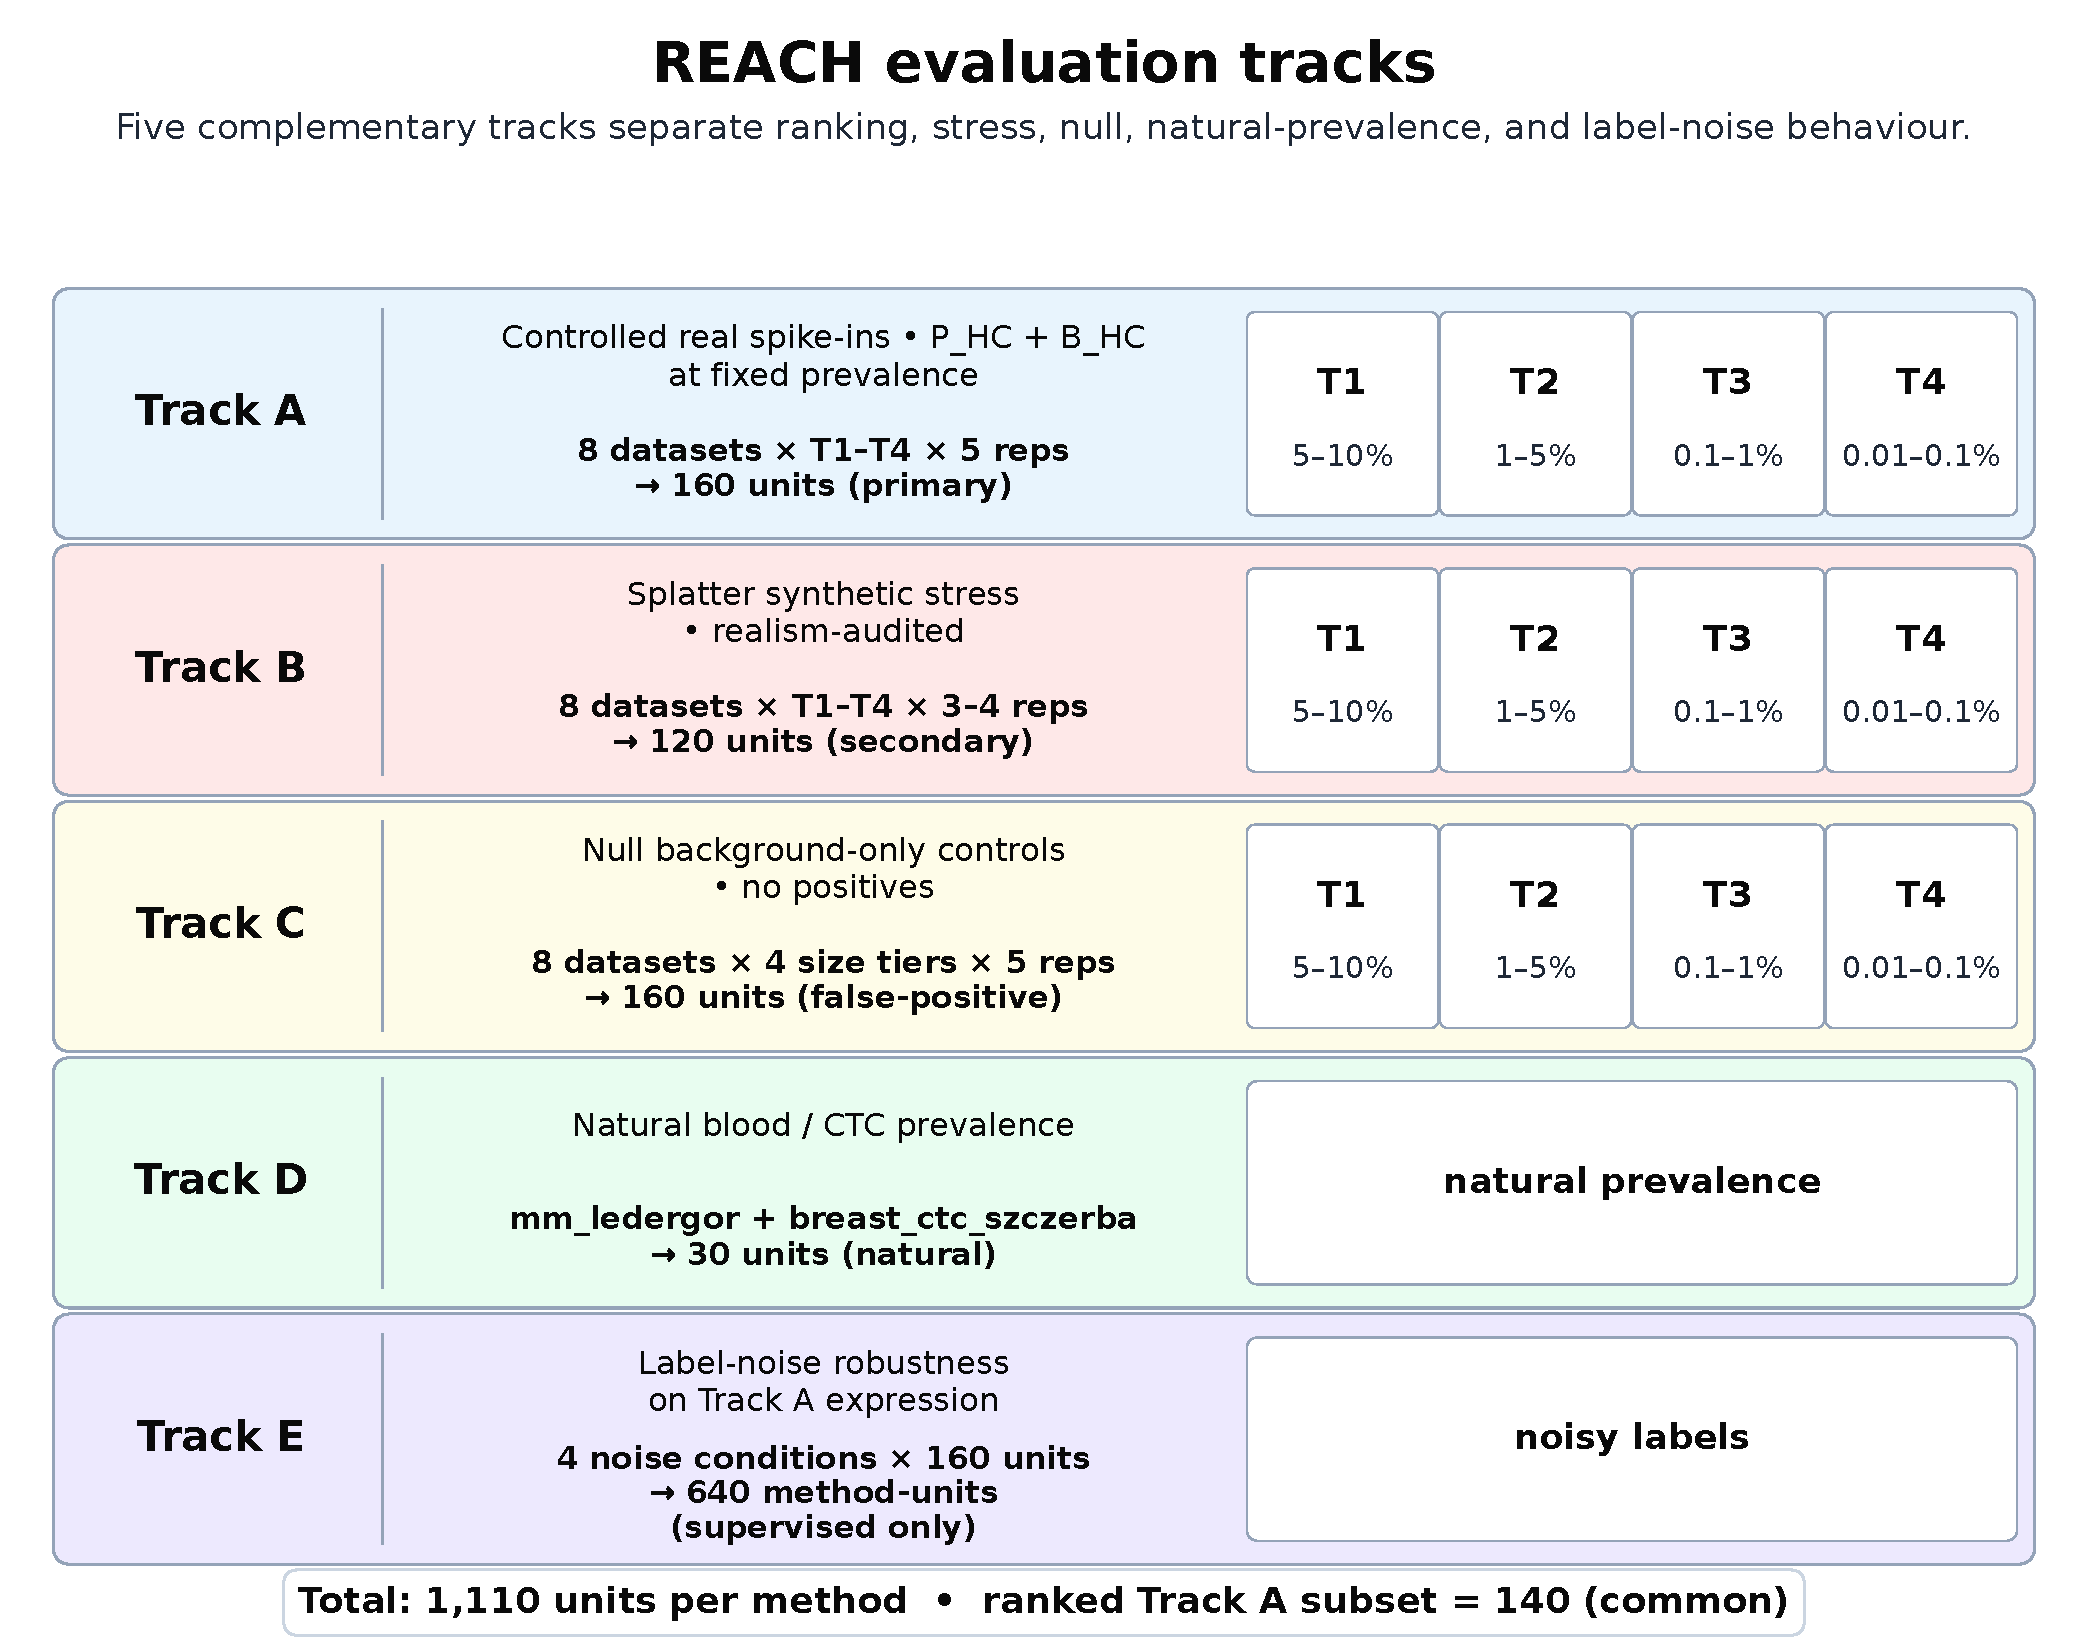
\includegraphics[
width=0.99\linewidth,
height=0.90\textheight,
keepaspectratio
]{figures_final/Fig2_Track_Design.pdf}
\caption{\textbf{REACH evaluation tracks.} Track~A controls real-cell
rarity across T1--T4 windows; Track~B tests synthetic stress; Track~C
exposes null/false-positive behavior; Track~D retains natural blood/CTC
prevalence; Track~E perturbs labels while holding expression fixed. There are
1{,}110 units per method total.}
\label{fig:tracks}
\end{figure}

\subsection{Method execution, score contracts, and QC}

The contract for a common wrapper run (input h5ad, output dir, config) will allow all of the methods to be executed in a single mode of operation. Each method wrapper produces a predictions.csv file containing cell-level scores and a runmeta.json file containing runtime, memory use, method version, success or failure status, fidelity status, and degenerate-output flags. Each of the methods will produce a quantitative (continuous variable) cell-based scoring of the cell sample, with the higher the score, the higher the evidence of the cell being a malignant or rare cell \cite{martens2023rarity,xu2024sccad}.


%-----------------------fig  3 ---------------------
\begin{figure}[H]
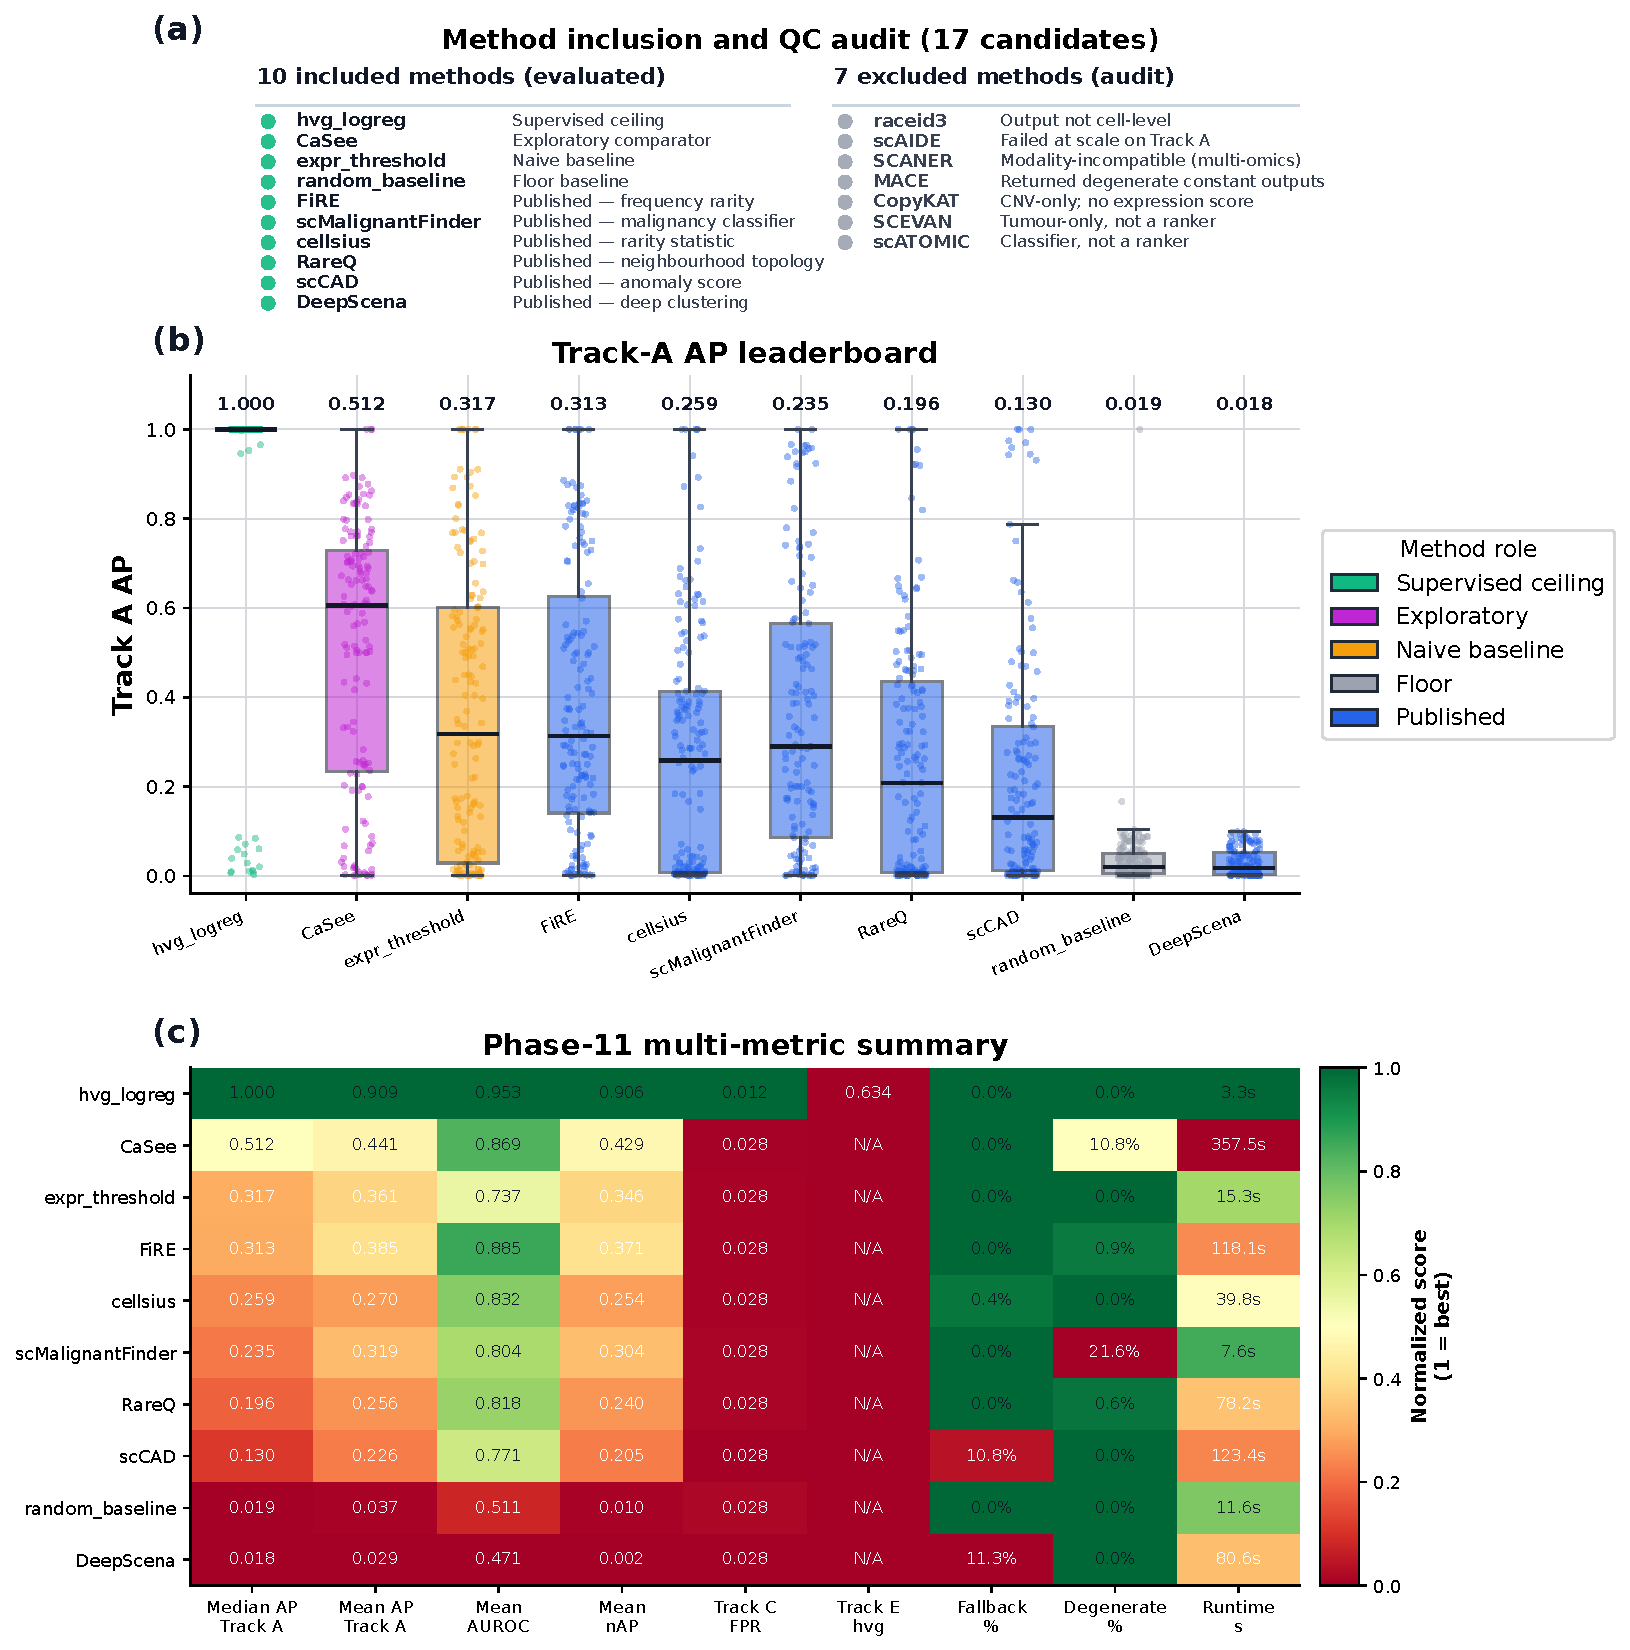
\includegraphics[
width=0.99\linewidth,
height=0.78\textheight,
keepaspectratio
]{figures_final/Fig3_Method_Audit_Leaderboard_Summary.pdf}
\caption{\textbf{Method audit, leaderboard, and multi-metric summary.}\\[4pt]
\label{fig:fig3}
\textbf{(a)} Method inclusion and QC audit. Seventeen candidate methods were considered. Ten produced evaluable outputs under the standardized score contract, while seven were excluded because of integration constraints, score-contract mismatch, out-of-memory or timeout failures, or degenerate outputs. The audit is part of the benchmark deliverable, not informal curation. \textbf{(b)} Track A AP leaderboard. Box-and-strip summaries show fallback-filtered Track A AP by method. The figure separates the supervised ceiling, exploratory comparator, naive baselines, ranked published methods, and random floor. \textbf{(c)} Phase 11 multi-metric summary heatmap. Min--max scaled values are shown across AP, nAP, AUROC, MCC at top-k, Track E robustness where applicable, runtime, and null-control behavior. The figure summarizes metric-level performance rather than dataset-by-method behavior.}

\end{figure}



REACH assesses ten of the included methods sorted by their interpretive role (Table 3). Method hvg-logreg is used as a supervised in-sample ceiling. It is not treated as an ordinary unsupervised detector; instead, it estimates how well malignant and background cells can be separated when label information is available. An exploratory comparator called CaSee is included, as it gives a cancer/normal scoring framework but again is not among the top ranked published detectors \cite{sh2022casee}. Main published ranked comparators in REACH include FiRE, DeepScena, RareQ, CellSIUS, scCAD and scMalignantFinder \cite{wegmann2019cellsius,xu2024sccad,yu2025scmalignantfinder}. Additionally, expr threshold and random baseline are provided as naive baselines: the former is a simple expression-based reference, while the latter provides a floor-level random baseline comparison. Methods that do not produce valid cell-level scores, exceed memory or runtime limits, or generate degenerate outputs are recorded in the method-inclusion audit and excluded from the main ranking analyses.


\begin{table}[H]
\centering
\caption{Audited unit counts per method per track. The total of 1{,}110
units yields 11{,}100 method-unit evaluations across ten included
methods.}
\label{tab:tracks}
\small
\begin{tabular}{llrl}
\toprule
Track & Purpose & Units & Primary interpretation \\
\midrule
A & Controlled real P\_HC spike-ins into B\_HC background & 160 & Primary ranked endpoint \\
B & Synthetic Splatter stress with realism audits         & 120 & Secondary stress test \\
C & Background dominated null controls                    & 160 & False positive behavior \\
D & Natural blood / CTC prevalence                        & 30  & Natural prevalence supplement \\
E & Track A expression with corrupted labels              & 640 & Supervised label noise analysis \\
\midrule
\multicolumn{2}{l}{\textit{Total}} & \textit{1{,}110} & \\
\bottomrule
\end{tabular}
\end{table}


\begin{table}[H]
\centering
\caption{Included methods and interpretive roles.}
\label{tab:methods}
\small
\begin{tabular}{llll}
\toprule
Method & Category & Output type & Role \\
\midrule
\texttt{random\_baseline}  & Naive       & Uniform random score                  & Floor baseline \\
\texttt{expr\_threshold}   & Naive       & Total UMI / signature expression rank & Naive biological baseline \\
\texttt{hvg\_logreg}       & Supervised  & Logistic probability on 2{,}000 HVGs   & In-sample ceiling \\
\texttt{FiRE}              & Ranked      & Frequency-based rarity score          & Published comparator \\
\texttt{DeepScena}         & Ranked      & Deep clustering / SSL score           & Published comparator \\
\texttt{RareQ}             & Ranked      & Neighborhood rarity score            & Published comparator \\
\texttt{cellsius}          & Ranked      & Rarity statistic                      & Published comparator \\
\texttt{scCAD}             & Ranked      & Anomaly score                         & Published comparator \\
\texttt{scMalignantFinder} & Ranked      & Malignancy probability                & Published / proxy comparator \\
\texttt{CaSee}             & Exploratory & Autoencoder $+$ Isolation Forest      & Exploratory faithful comparator \\
\bottomrule
\end{tabular}
\end{table}

Fallback scores arise when a wrapper
returns random scores after timeout or memory failure; these units are
\emph{filtered out} of AP aggregation. Degenerate scores are constant or near constant outputs; these are retained, flagged, and reported.
Here, the audited snapshot contains 249 fallback units across
methods (DeepScena~125, scCAD~120, cellsius~4) and 377 degenerate units
(scMalignantFinder~240, CaSee~120, FiRE~10, RareQ~7).

\subsection{Reproducible extension protocol}

REACH is extensible. If users want to add a new method, then they have to implement the wrapper which follows the standard REACH run contract and register that method in the method registry. Basic metadata and a smoke test that identifies it can run correctly must be included within each method before being added to the overall benchmark. Output from the system is designed to be very simple: a score (at cell level), an optional predicted label, runtime metadata, fidelity and fallback or degenerate flags.

We can also add new datasets, which involves creating a dataset-registry entry, raw-data loader, source-annotation mapper, signature configuration, preprocessing outputs and the corresponding Track A--E benchmark units. Likewise, to add a new evaluation track or metric, one needs to provide updates on the appropriate track generator, evaluator (wherever it is defined), aggregation tables and figure-generation scripts \cite{everingham2010pascal,abdelaal2019comparison,tran2020benchmark}.

% ----------EXPERIMENTS SECTION 4-------------
\section{Experiments}

\subsection{Benchmark scale}

Across ten methods, REACH evaluates 1,110 benchmark units per method, resulting in 11,100 method-unit evaluations \cite{abdelaal2019comparison,abdelaal2025benchmarking}. The primary leaderboard displays median AP on Track A after method specific fallback filtering. The global rank test and pairwise rank test use the 140 unit common subset of Track A retained after method specific fallback filtering, with 2,000 bootstrap resamples calculated for rank intervals \cite{cao2021benchmark}.

\subsection{Statistical testing}

A Friedman test with Iman-Davenport correction was used to assess global differences in per-unit Track A AP across methods \cite{gorodkin2004comparing}. Wilcoxon signed rank tests against the top published method (FiRE) were performed for each pairwise comparison, with Benjamini-Hochberg FDR correction. However, these corrections are not reported at all unless the relevant repository table is provided. Where appropriate, mean differences and Cliff’s $\delta$ define the effect size of method comparisons. Rank uncertainty estimates are derived from 2{,}000 bootstrap resamples (rank ci.csv). Rarity sensitivity is assessed by regressing nAP against $\log_{10} \pi_u$ \cite{saito2015precision,davis2006relationship}.

% --------------RESULTS SECTION 5-----------
\section{Results}

\subsection{Primary Track A leaderboard}

The primary leaderboard is grouped by the median AP following the fallback filter (Table 4 and Fig.~\ref{fig:fig3}(b)). The median AP of 1.00 for hvg-logreg indicates that many high confidence malignant and background labels contain gene expression differences that can be recovered by a supervised model \cite{stegle2015computational,ren2018understanding}.

CaSee is ranked as the second highest median AP (0.512), but it is reported as an exploratory faithful comparator rather than as a primary ranked published detector among the published methods \cite{sh2022casee}. FiRE has the highest median AP (0.313) of any ranked published comparators. The naive expr-threshold baseline is slightly larger than the median AP (0.317) but is not presented as a published detector. The reported median of the naïve expr-threshold is greater than FiRE's and is to be interpreted as a caution that a naïve approach to the expression burden may be competitive in some cancers (\textit{i.e.}, naïve threshold expressed in earlier reports) \cite{torre2018rare}.

\begin{table}[H]
\centering
\caption{Primary Track A performance from \texttt{statistical\_ranking.csv}.
Runtime is the mean Track A wall clock time. The supervised ceiling and
exploratory comparator are not ordinary unsupervised leaderboard
entries.}
\label{tab:leaderboard}
\small
\begin{tabular}{llrrrrl}
\toprule
Role rank & Method & Median AP & Mean AP & AUROC & Runtime (s) & Role \\
\midrule
--   & \texttt{hvg\_logreg}        & \textbf{1.000} & 0.909 & 0.953 & 3.3   & Supervised ceiling \\
--   & \texttt{CaSee}              & 0.512          & 0.441 & 0.869 & 357.5 & Exploratory \\
--   & \texttt{expr\_threshold}    & 0.317          & 0.361 & 0.737 & 15.3  & Naive baseline \\
1    & \texttt{FiRE}               & 0.313          & 0.385 & 0.885 & 118.1 & Published \\
2    & \texttt{cellsius}           & 0.259          & 0.270 & 0.832 & 39.8  & Published \\
3    & \texttt{scMalignantFinder}  & 0.235          & 0.319 & 0.804 & 7.6   & Published / proxy \\
4    & \texttt{RareQ}              & 0.196          & 0.256 & 0.818 & 78.2  & Published \\
5    & \texttt{scCAD}              & 0.130          & 0.226 & 0.771 & 123.4 & Published \\
--   & \texttt{random\_baseline}   & 0.019          & 0.037 & 0.511 & 11.6  & Floor baseline \\
6    & \texttt{DeepScena}          & 0.018          & 0.029 & 0.471 & 80.6  & Published \\
\bottomrule
\end{tabular}
\end{table}

\subsection{Multi metric summary and dataset heterogeneity}

 Heatmaps of Phase 11 (Fig.~\ref{fig:fig3}(c)) reveal trade-offs between methods for all APs, nAPs, AUROC and MCC at the top of each list (and sometimes Track E robustness) as well as for runtime and null control behavior for all methods tested. There is no overall winner in all categories \cite{wang2022comparison,brendel2022application}. The best datasets vary (Table 5): CaSee is the best on 4 datasets (bcc yost, pdac peng, luad laughney, and hcc wei); expr-threshold is the best on 2 datasets (hnscc puram and ov izar tirosh). On the other hand, cellsius is the best on 1 dataset (rcc multi), whereas scMalignantFinder is the best on 1 dataset (crc lee). This variability justifies reporting method performance according to the context (tumor type) rather than a ``best method" story \cite{peng2019single,qian2020pan,tirosh2024cancer}.
%------------------fig 5--------------------------

\begin{table}[H]
\centering
\caption{Best overall and best non ceiling method by dataset, copied
from \texttt{best\_model\_per\_dataset.csv}. Non ceiling includes
exploratory and naive comparators.}
\label{tab:bestdataset}
\small
\begin{tabular}{llrlr}
\toprule
Dataset & Best overall & AP & Best non ceiling & AP \\
\midrule
\texttt{bcc\_yost}        & \texttt{hvg\_logreg}     & 1.0000 & \texttt{CaSee}             & 0.6079 \\
\texttt{hnscc\_puram}     & \texttt{hvg\_logreg}     & 1.0000 & \texttt{expr\_threshold}   & 0.7872 \\
\texttt{pdac\_peng}       & \texttt{hvg\_logreg}     & 1.0000 & \texttt{CaSee}             & 0.4488 \\
\texttt{rcc\_multi}       & \texttt{hvg\_logreg}     & 1.0000 & \texttt{cellsius}          & 0.1931 \\
\texttt{crc\_lee}         & \texttt{hvg\_logreg}     & 0.9998 & \texttt{scMalignantFinder} & 0.8373 \\
\texttt{luad\_laughney}   & \texttt{hvg\_logreg}     & 0.9983 & \texttt{CaSee}             & 0.5378 \\
\texttt{hcc\_wei}         & \texttt{hvg\_logreg}     & 0.9948 & \texttt{CaSee}             & 0.4908 \\
\texttt{ov\_izar\_tirosh} & \texttt{expr\_threshold} & 0.5717 & \texttt{expr\_threshold}   & 0.5717 \\
\bottomrule
\end{tabular}

\end{table}

\subsection{Statistical significance and rank uncertainty}

The overall rank tests have been conducted on the 140 common unit Track A subset. These tests showed significant differences across methods: Friedman $\chi^2 = 695.05$, $p < 0.001$; Iman-Davenport $F = 171.01$, $p < 0.001$ \cite{davis2006relationship,saito2015precision}. The results of the pairwise Wilcoxon tests relative to FiRE (Table 6) suggest that FiRE has significantly better performance than random baseline, DeepScena, scCAD, RareQ and cellsius ($p < 0.05$ after Benjamini-Hochberg FDR correction). There are no significant differences between scMalignantFinder and expr threshold methods when compared to FiRE. In our exploratory comparison, CaSee is better than FiRE ($\Delta$mean AP = $-0.140$, BH FDR = $6.1 \times 10^{-8}$; Cliff’s $\delta = -0.245$); this is reported under the exploratory versus published category, not under the primary ranked method category \cite{sh2022casee}.

\begin{table}[H]
\centering
\caption{Selected pairwise comparisons on Track A AP from
\texttt{pairwise\_tests.csv}. Positive $\Delta$ means \texttt{FiRE} has
higher mean AP than the comparator; negative $\Delta$ means the
comparator has higher mean AP.}
\label{tab:pairwise}
\small
\begin{tabular}{lrrrr}
\toprule
Comparator & $\Delta$ mean AP & Wilcoxon $p$ & BH FDR & Cliff's $\delta$ \\
\midrule
\texttt{DeepScena}        &  0.3320 & $1.10\!\times\!10^{-24}$ & $1.66\!\times\!10^{-23}$ &  0.7539 \\
\texttt{random\_baseline} &  0.3226 & $2.52\!\times\!10^{-22}$ & $8.11\!\times\!10^{-22}$ &  0.7271 \\
\texttt{CaSee}            & -0.1395 & $3.96\!\times\!10^{-8}$  & $6.14\!\times\!10^{-8}$  & -0.2451 \\
\texttt{scCAD}            &  0.1350 & $1.56\!\times\!10^{-4}$  & $2.34\!\times\!10^{-4}$  &  0.2886 \\
\texttt{RareQ}            &  0.1161 & $1.77\!\times\!10^{-3}$  & $2.49\!\times\!10^{-3}$  &  0.2457 \\
\texttt{cellsius}         &  0.0978 & $3.06\!\times\!10^{-3}$  & $4.04\!\times\!10^{-3}$  &  0.1930 \\
\texttt{scMalignantFinder}&  0.0453 & 0.812                    & 0.831                    &  0.1206 \\
\texttt{expr\_threshold}  &  0.0304 & 0.836                    & 0.836                    &  0.0816 \\
\bottomrule
\end{tabular}
\end{table}

The bootstrap intervals for ranks are stable, whereas the hvg logreg and CaSee methods are ranked 1 and 2 respectively for every resample of 2,000. On the other hand, FiRE is observed to have a median rank of 3 (with a 95\% bootstrap rank interval of [3, 4]). Expr threshold, scMalignantFinder, cellsius, RareQ, and scCAD fall into an overlapping middle band (Fig.~\ref{fig:fig4}(a)). The mean within-unit rank for each method, shown in Fig.~\ref{fig:fig4}(b), separates the strongest methods from the overlapping middle group and is consistent with the bootstrap rank intervals \cite{gorodkin2004comparing}.

\subsection{Rarity sensitivity and track specific robustness}
Rarity sensitivity was assessed by regressing nAP against $\log_{10}(\pi_u)$, where $\pi_u$ denotes the positive-cell prevalence in each benchmark unit (Fig.~\ref{fig:fig4}(c)). Most methods show positive slopes, indicating that performance improved as rare cells became less sparse. CellSIUS shows the largest nAP slope ($0.220$, $p = 1.78 \times 10^{-20}$), while RareQ, CaSee, scMalignantFinder, scCAD, FiRE, and expr threshold show similar positive slopes. These nAP slopes are descriptive \cite{johnson2019survey,altalhan2025imbalanced}.

There is a reordering of methods in Track B versus Track A (Spearman rank correlation $\rho = 0.042$, $p = 0.907$, so the Track B stands as a stress test versus being incorporated into the primary leaderboard (Fig.~\ref{fig:fig5}(a), left side) \cite{cao2021benchmark}. The track E hvg-logreg label noise analysis shows that the loss in mean AP is relative to a Track A mean AP of $0.9088$: hvg-logreg mean AP drops between $0.909$ and $0.534$ under $30\% $ background-to-positive flips, $0.829$ under $30\%$ positive to background flips, $0.481$ under $10\%$ symmetric noise and $0.460$ under $20\%$ symmetric noise. On the other hand, the corresponding robustness indices (ranging from 0 to 1) for these analyses are $0.588$, $0.912$, $0.529$, $0.507$ respectively (Fig.~\ref{fig:fig5} (a), right side) \cite{mahalanabis2022evaluation}.

\subsection{Null behavior and calibration}

Track C evaluates false-positive behavior in background dominated units, where no true rare malignant cells are expected (Fig.~\ref{fig:fig5}(b)) \cite{torre2018rare}. For each method, REACH measures the fraction of top ranked cells that are incorrectly selected as positives under these null-control conditions. Most unsupervised, exploratory, and naive scoring methods show an average top k false positive rate of approximately 3\%: CaSee = 0.0301, DeepScena = 0.0306, FiRE = 0.0315, RareQ = 0.0293, CellSIUS = 0.0295, expr-threshold = 0.0310, scCAD = 0.0301, scMalignantFinder = 0.0315, and random baseline = 0.0309. In contrast, the supervised hvg-logreg ceiling shows a much higher Track C false positive rate of 0.788. This behavior is expected because hvg-logreg is an in-sample supervised ceiling, not a deployable unsupervised detector. Calibration has been assessed only for methods that produced probability-like scores \cite{christensen2023evaluation,abdelaal2019comparison}.

\subsection{Runtime, scalability, and failure modes}

Runtime varies by approximately two orders of magnitude across methods (Fig.~\ref{fig:runtime}). Track A Mean Execution Times (MET) for the corresponding tools range from 3.3 seconds (hvg-logistic regression) to 7.6 seconds (scMalignantFinder) to 357.5 seconds (CaSee); FiRE MET of 118.1 seconds, scCAD MET of 123.4 seconds, RareQ MET of 78.2 seconds, DeepScena MET of 80.6 seconds, cellsius MET of 39.8 seconds \cite{brendel2022application,wang2022comparison}. Runtime also needs to be put into context with fallback and/or degenerate output behavior. Runtime should therefore be interpreted together with fallback and degenerate-output rates, because a fast method is not necessarily reliable if it frequently returns constant scores or fails on many benchmark units \cite{everingham2010pascal,tran2020benchmark}.


\begin{figure}[H]
\centering
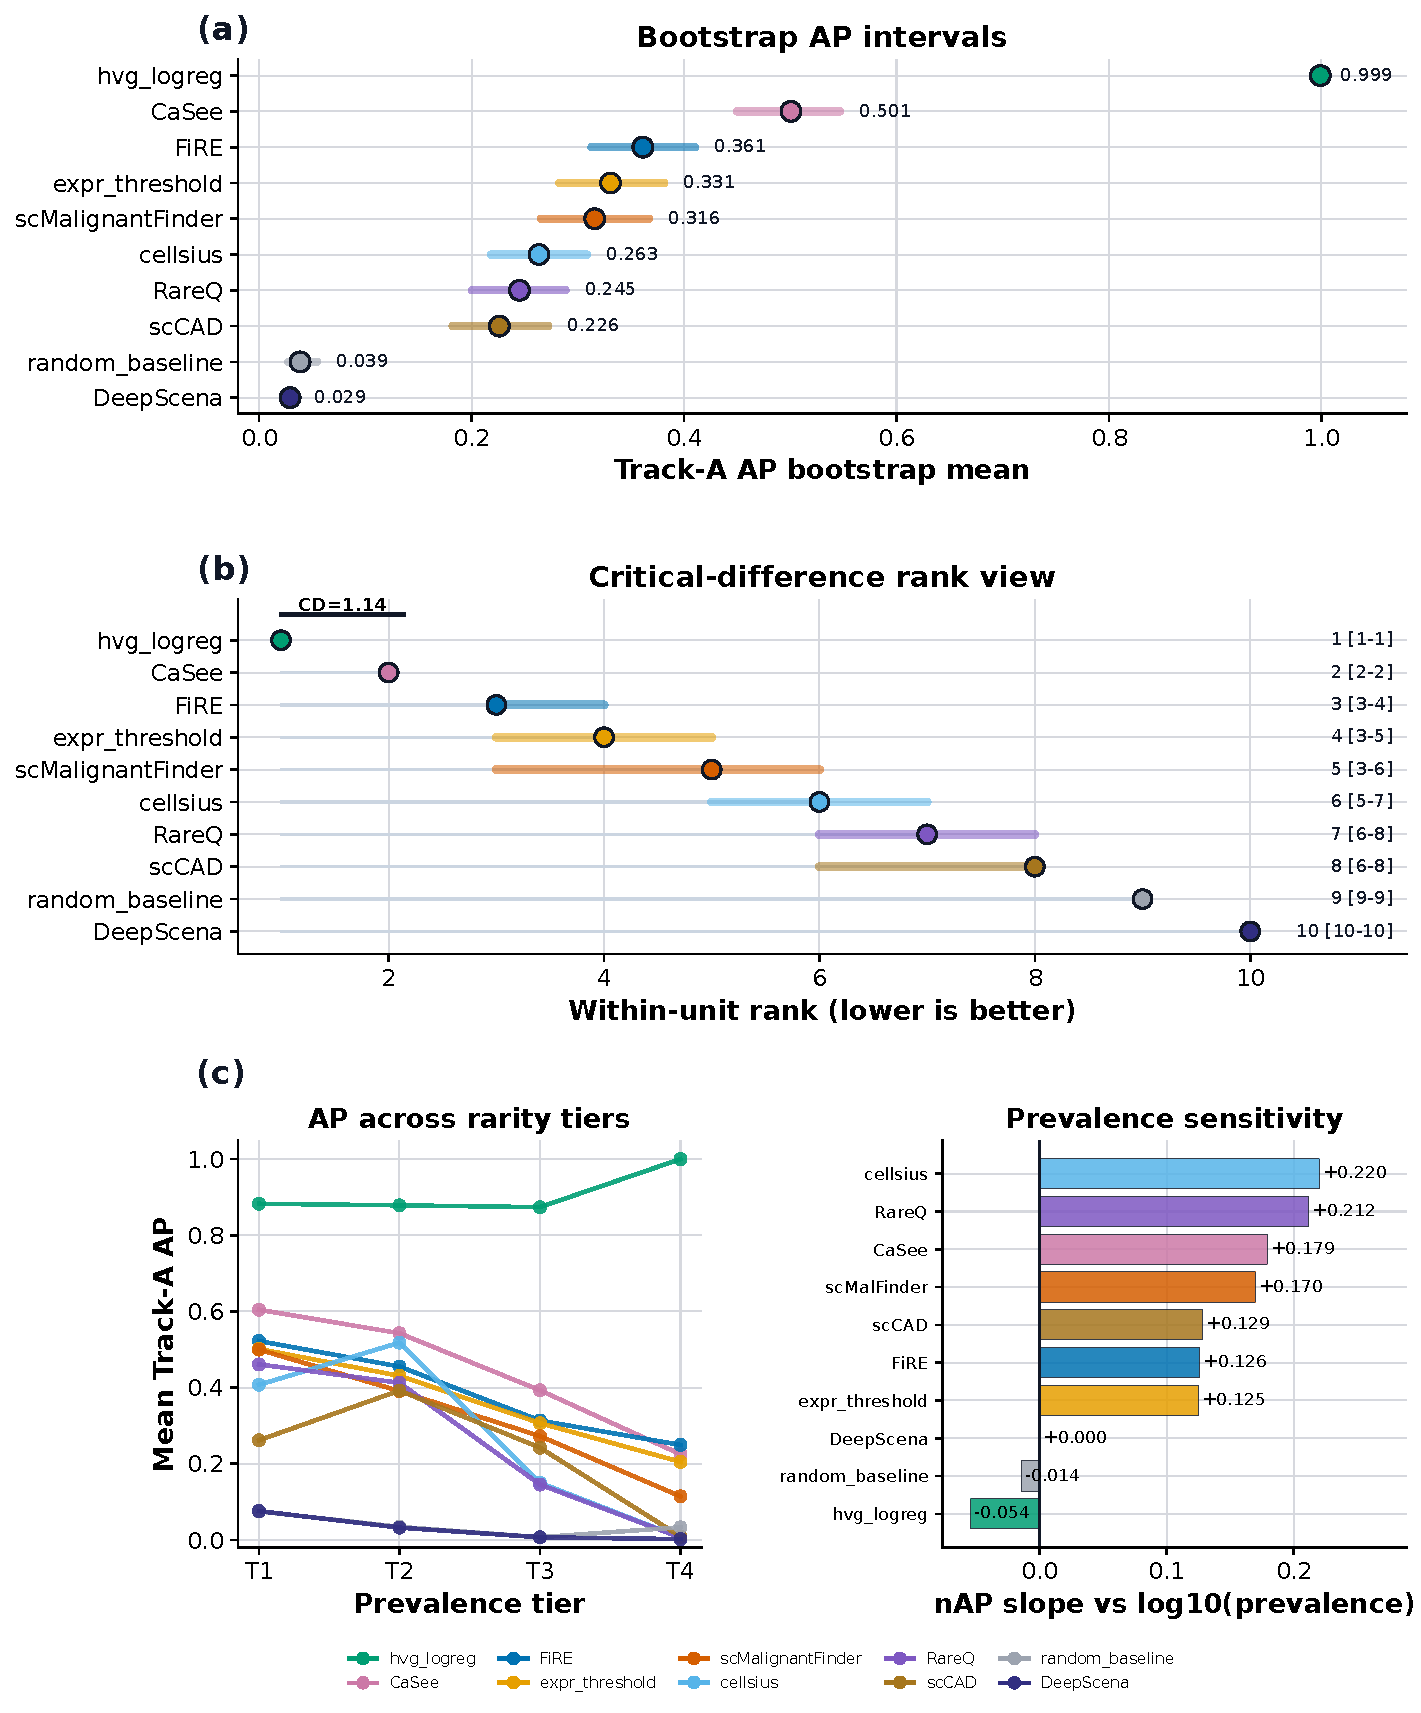
\includegraphics[
width=0.95\linewidth,
height=0.78\textheight,
keepaspectratio
]{figures_final/Fig4_Rank_Uncertainty_Rarity.pdf}
\caption{\textbf{Rank uncertainty, critical difference, and rarity sensitivity.}\\[4pt]
\textbf{(a)} Bootstrap rank confidence intervals. Ranks are computed from Track A AP over 2{,}000 unit level bootstrap resamples (\texttt{rank\_ci.csv}). Lower rank is better. \textbf{(b)} Critical difference rank view. It shows the mean within unit ranks on the common Track A subset, with the Nemenyi critical difference bar (CD$\,\approx\,1.14$, $k=10$, $N=140$, $\alpha=0.05$). \textbf{(c)} Rarity sensitivity. It depicts AP and normalized AP across Track A prevalence tiers T1--T4. Several methods degrade sharply in ultra rare units, while the supervised ceiling remains near $1$ across tiers.}

\label{fig:fig4}
\end{figure}

\begin{figure}[H]
\centering
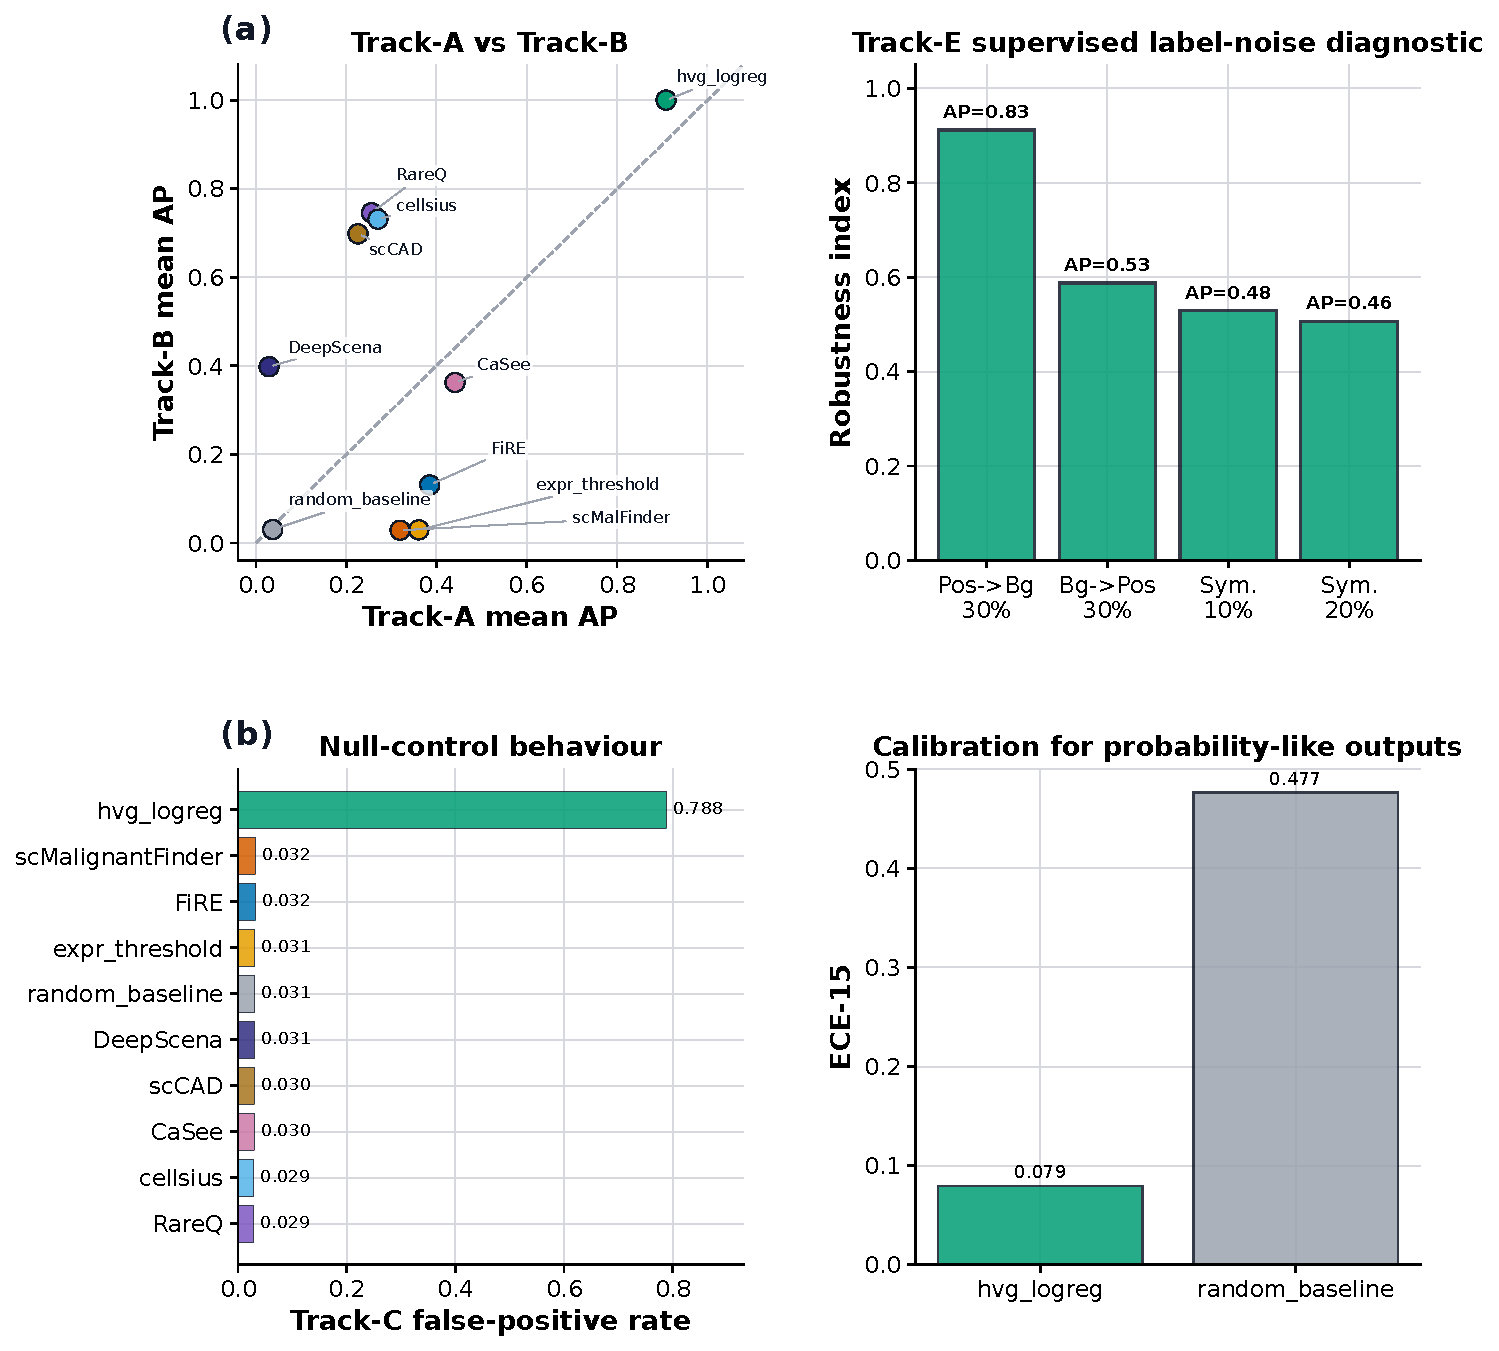
\includegraphics[
width=0.95\linewidth,
height=0.78\textheight,
keepaspectratio
]{figures_final/Fig5_Track_Sensitivity_Null.pdf}
\caption{\textbf{Track sensitivity, robustness, and null behavior.}\\[4pt]
\textbf{(a)} Track sensitivity and supervised label noise diagnostics. Left: Track A vs Track B mean AP per method, with the diagonal showing equal performance. Right: Track E robustness indices for the supervised ceiling under four label perturbations. Track~E is not interpretable for unsupervised methods.\\[3pt]
\textbf{(b)} Track C null behavior and calibration. Background dominated units assess false positive behavior. ECE is shown only for methods with probability like outputs.}

\label{fig:fig5}
\end{figure}

\section{Discussion}

REACH shows a clear gap between supervised separability and the performance of current unsupervised rare malignant-cell ranking methods \cite{abdelaal2019comparison,christensen2023evaluation}. The supervised hvg-logreg ceiling indicates that many high confidence malignant and background labels contain recoverable gene expression differences. In other words, when label information is available, these cell groups can often be separated with very high accuracy. However, the lower Track A AP values obtained by unsupervised and rarity-based methods show that current scoring approaches recover only part of this separability \cite{lei2023self,martens2023rarity}. This gap is important because rare malignant cell detection is not only a question of whether the signal exists in the data, but also whether an unsupervised method can reliably recover it under strong class imbalance and tumor heterogeneity.

The results also support the need for a multi track benchmark rather than a single leaderboard. Track A provides the primary evaluation under controlled real-cell rarity. Track B tests whether methods remain stable under synthetic stress, but its ranking does not reproduce Track A and therefore should not be averaged into the primary leaderboard. Track C adds a null control setting to examine false-positive behavior when malignant cells are not expected. Track D preserves natural prevalence in blood and circulating tumor cell datasets. Track E evaluates the effect of label corruption on the supervised ceiling and should not be interpreted as evidence of unsupervised robustness \cite{cao2021benchmark,torre2018rare,mahalanabis2022evaluation}. Together, these tracks show that different evaluation conditions reveal different aspects of method behavior.

The main practical message from REACH is that method performance should be interpreted with caution. FiRE is the strongest ranked published comparator on the primary Track A endpoint, but its advantage is not uniform across all comparisons. In the paired tests, FiRE is not significantly better than the naive expr-threshold baseline or scMalignantFinder. CaSee performs better than FiRE in the exploratory comparison, but it is substantially slower and produces constant scores in some benchmark units \cite{sh2022casee,yu2025scmalignantfinder}. Dataset level results also show that different methods perform best in different tumor contexts. Therefore, REACH does not support the idea of a single universally best method. Instead, rare malignant cell detection methods should be reported together with the dataset context, prevalence level, failure behavior, and the evaluation track in which they were tested \cite{peng2019single,qian2020pan,tirosh2024cancer}.

\begin{figure}[H]
\centering

\includegraphics[
width=0.95\linewidth,
height=0.78\textheight,
keepaspectratio
]{figures_final/Fig6_Runtime_Scalability_Pareto.pdf}
\caption{\textbf{Runtime and AP Pareto behavior.} Left: per unit
runtime versus cells per unit. Right: mean Track A runtime versus mean
Track A AP, highlighting the trade off between ranking performance,
compute cost, and method stability.}
\label{fig:runtime}
\end{figure}

\section{Limitations}

This study has a few limitations that should be considered when interpreting the results. First, CNV evidence in the current version of REACH was generated using infercnvpy as the primary CNV inference approach. CopyKAT was not used as a primary scored comparator because it did not satisfy the uniform cell-level score contract and could not be applied consistently across all datasets. This means that CNV evidence was handled consistently within the benchmark, but it was not independently cross-validated using a second CNV caller \cite{chen2025benchmarking,gao2021delineating}.

Second, the current dataset collection does not yet cover the full diversity of cancer scRNA-seq data. Most datasets are based on 10x Chromium technology, while only two datasets are based on Smart-seq2. Spatial transcriptomics, multi-omics datasets, and a wider range of tumor types are not included in this version \cite{jovic2022single}. Therefore, the present results should be viewed as a first benchmark snapshot rather than a complete evaluation of all possible rare malignant-cell detection settings.

Third, some degree of circularity may remain in the label construction. Because CNV evidence contributes to the definition of high-confidence malignant cells, methods that indirectly capture CNV-related expression patterns may benefit in some datasets. This is particularly relevant for datasets such as \textit{ov\_izar\_tirosh}, where CNV-supported labelling contributes to the evidence used for defining malignant cells. Future versions of REACH should reduce this limitation by comparing multiple CNV callers and by testing label definitions that are less dependent on a single evidence source.

Fourth, Track E has a limited interpretation. It is useful for examining how the supervised hvg-logreg ceiling responds to corrupted labels, but it should not be interpreted as a general robustness test for unsupervised rare-cell detection methods. This distinction is important because unsupervised methods do not use label information in the same way as the supervised ceiling.

Fifth, method stability remains an important practical issue. In the current benchmark, 249 fallback units and 377 degenerate units were recorded. These failures show that some methods still face difficulties related to memory use, runtime limits, wrapper stability, or constant score outputs. For rare-cell detection benchmarks, reliability is therefore as important as accuracy: a method that performs well in some units but fails in many others may not be practically useful \cite{tran2020benchmark,everingham2010pascal}.

Finally, public leaderboards can create a risk of overfitting. If methods are repeatedly tuned on the same visible datasets and tracks, leaderboard performance may not reflect general performance on unseen data. Future versions of REACH should include hidden test datasets, pre-registered track definitions, post-submission perturbation tracks, and containerized execution with fixed prediction schemas. The aforementioned changes could make the benchmark more robust and more useful for evaluating new rare malignant-cell detection methods \cite{song2023benchmarking,li2023comprehensive}.

\section{Conclusion}

REACH offers a reproducible way to compare methods for detecting rare malignant cells in scRNA-seq data. The benchmark is designed around the practical difficulties of this task: rare cells are often present at very low frequency, their labels may require more than one source of evidence, and method outputs can vary across datasets and tumor contexts. To address these issues, REACH combines multi evidence high confidence labels, controlled and natural prevalence settings, null controls, label noise analysis, fallback-aware metrics, statistical testing, and reproducible figure generation from audited results.

The current benchmark shows that rare malignant cell detection remains challenging. The supervised hvg-logreg ceiling performs strongly on Track A, suggesting that many high confidence malignant and background cells can be separated using gene expression information. However, current unsupervised and rarity-based methods recover only part of this separation. Among the ranked published methods, FiRE gives the strongest performance on the primary Track A endpoint, while CaSee provides a strong exploratory comparison but should not be treated as an ordinary ranked published detector. The results also indicate that the best performing method changes from one dataset to another, suggesting that no single method is consistently best across all tumor contexts.

These findings support the need for careful, context specific benchmarking. Instead of reducing performance to one overall leaderboard, REACH encourages results to be interpreted together with tumor type, rarity level, false-positive behavior, method stability, and evaluation track. In this sense, REACH provides a transparent platform for future method comparison and a practical reference for developing more robust and reproducible rare malignant cell detection methods.

\section*{Data and Code Availability}

The REACH benchmark framework, including all source code, pipelines, and evaluation scripts, is publicly available at: \url{https://github.com/jaswanthmoram/reach-rarecell-benchmark}. Versioned Zenodo archives containing the processed datasets, benchmark units, and result tables are available with the latest release.
All datasets used in this project have been obtained from public databases, specifically the GEO, and all sources are cited within the manuscript. The processed dataset, along with benchmark units and performance results, will also be available with the repository.
The GitHub repository includes toy workflows, scripts for deterministic snapshot regeneration, and documentation for reproducing the benchmark using the archived data and specified compute environment. All results/figures reported in this analysis can be regenerated deterministically from any prediction output stored using the scripts provided. All environment specifications are thoroughly documented in order to achieve reproducibility across computational environments.

\section*{Acknowledgements}

\nocite{*}
\bibliographystyle{unsrt}
\bibliography{references/master}
\end{document}